% Results
\section{Results}
\label{sec:results}

We organize results around eight claims.

\subsection{Claim 1: ISR changes the selected basin}

Table~\ref{tab:main_distribution} shows the final probability distributions at
$N = 10,\!000$. The global census favors vacuum~2 by raw count, while
\ISR (Gaussian $\ell = 1$) shifts weight toward vacuum~3, the basin
containing $x_0$.

\begin{table}[t]
  \centering
  \caption{Probability distribution over vacuum basins at final cutoff $N=10000$. ISR uses a Gaussian kernel with $\ell=1$. Metrics: KL drift $=3.58\times10^{-4}$ (global) vs $1.27\times10^{-4}$ (ISR); Wasserstein $=9.30\times10^{-3}$ vs $6.41\times10^{-3}$; both measures are stable under cutoff extension.}
  \label{tab:main_distribution}
  \begin{tabular}{lccc}
    \toprule
    Vacuum & Global census & ISR Gaussian $\ell=1$ & Difference \\
    \midrule
    0 & 0.000700 & 0.000000 & -0.000700 \\
    1 & 0.044000 & 0.000207 & -0.043793 \\
    2 & 0.396000 & 0.264742 & -0.131258 \\
    3 & 0.358600 & 0.661812 & +0.303212 \\
    4 & 0.186600 & 0.073217 & -0.113383 \\
    5 & 0.014100 & 0.000023 & -0.014077 \\
    \bottomrule
  \end{tabular}
\end{table}


Fig.~\ref{fig:global_vs_isr} visualizes this shift.
The global census allocates 39.6\% to vacuum~2 and 35.9\% to vacuum~3.
\ISR reverses this: vacuum~2 falls to 26.5\% while vacuum~3 rises to 66.2\%.

\begin{figure}[t]
  \centering
  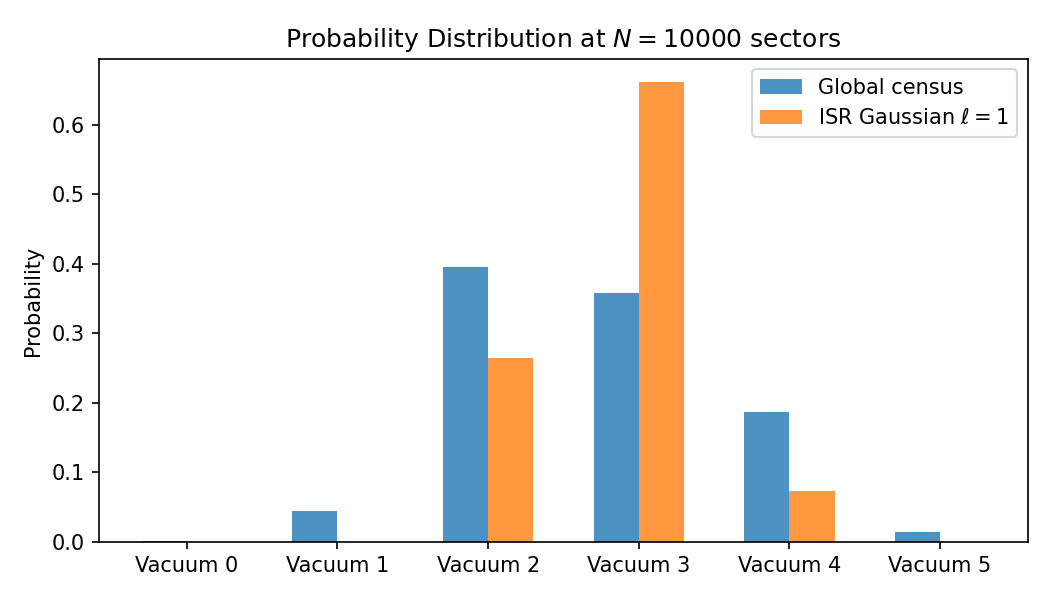
\includegraphics[width=\columnwidth]{figures/fig_02_global_vs_isr_distribution.png}
  \caption{Probability distribution at $N = 10,\!000$ sectors.
  \ISR shifts weight from the most populous vacuum~2 to the local vacuum~3.}
  \label{fig:global_vs_isr}
\end{figure}

\subsection{Claim 2: ISR improves finite-sample cutoff stability}

Table~\ref{tab:main_distribution} shows that \ISR reduces the final KL drift
from $3.58\times10^{-4}$ (global census) to $1.27\times10^{-4}$ (ISR),
an improvement by approximately a factor of two.
The Wasserstein distance improves from $9.30\times10^{-3}$ to $6.41\times10^{-3}$.
Fig.~\ref{fig:kl_drift} compares the two measures.

\begin{figure}[t]
  \centering
  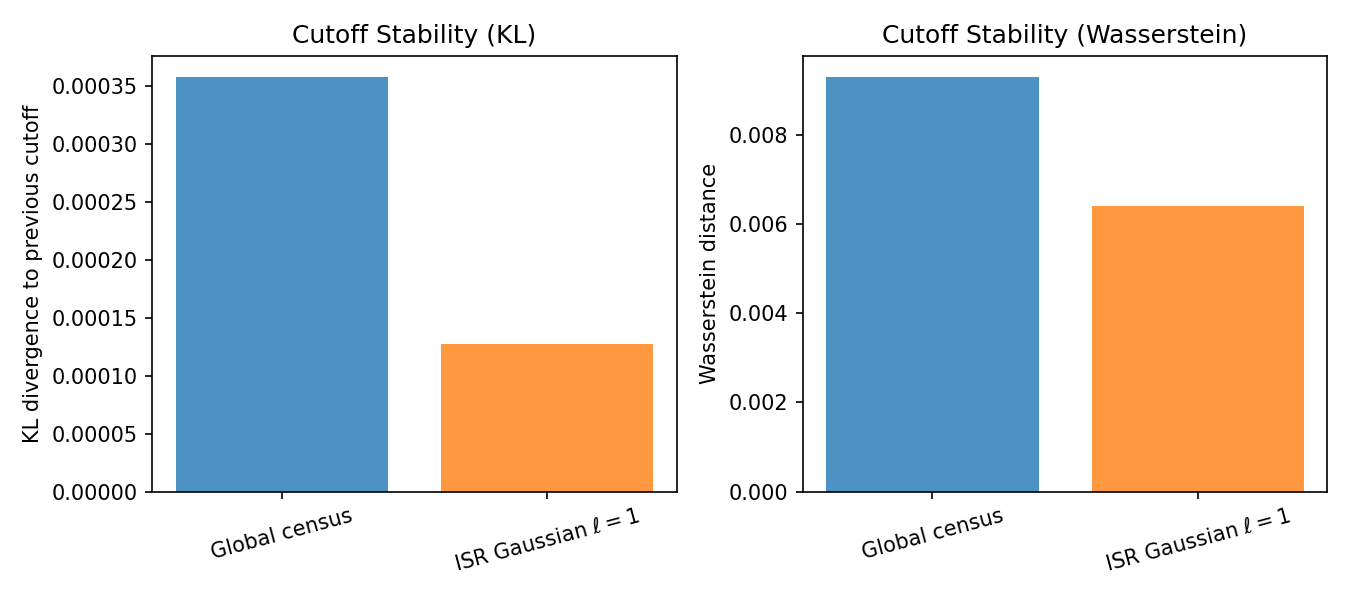
\includegraphics[width=\columnwidth]{figures/fig_03_kl_drift_global_vs_isr.png}
  \caption{KL divergence and Wasserstein distance for global census and
  \ISR (Gaussian $\ell = 1$) at $N = 10,\!000$.
  \ISR reduces both metrics.}
  \label{fig:kl_drift}
\end{figure}

\subsection{Claim 3: ISR is robust across stress tests}

Table~\ref{tab:stress_summary} summarizes the 100-run stress test.
\ISR improves over global census in 98 of 100 runs.
The improvement ratio is largest at intermediate $\sigma$ values
($1.0$--$2.0$), where the initial-condition spread samples multiple basins
but remains concentrated enough for locality weighting to be effective.

\begin{table}[t]
  \centering
  \caption{Stress test summary by $\sigma$. Each row aggregates 20 random seeds with $N=2000$ trajectories per run.}
  \label{tab:stress_summary}
  \begin{tabular}{lcccccc}
    \toprule
    $\sigma$ & Global mean KL & ISR mean KL & Median improv. & ISR wins / total & Mean $n_{\rm vacua}$ \\
    \midrule
    0.5 & 0.0008 & 0.0003 & 2.1$\times$ & 20/20 & 3.0 \\
    1.0 & 0.0013 & 0.0003 & 3.9$\times$ & 20/20 & 4.7 \\
    1.5 & 0.0012 & 0.0003 & 4.7$\times$ & 20/20 & 6.0 \\
    2.0 & 0.0011 & 0.0003 & 3.7$\times$ & 20/20 & 6.0 \\
    3.0 & 0.0010 & 0.0004 & 3.4$\times$ & 18/20 & 6.0 \\
    \bottomrule
  \end{tabular}
\end{table}


Fig.~\ref{fig:stress_improvement} shows the distribution of improvement ratios
by $\sigma$.

\begin{figure}[t]
  \centering
  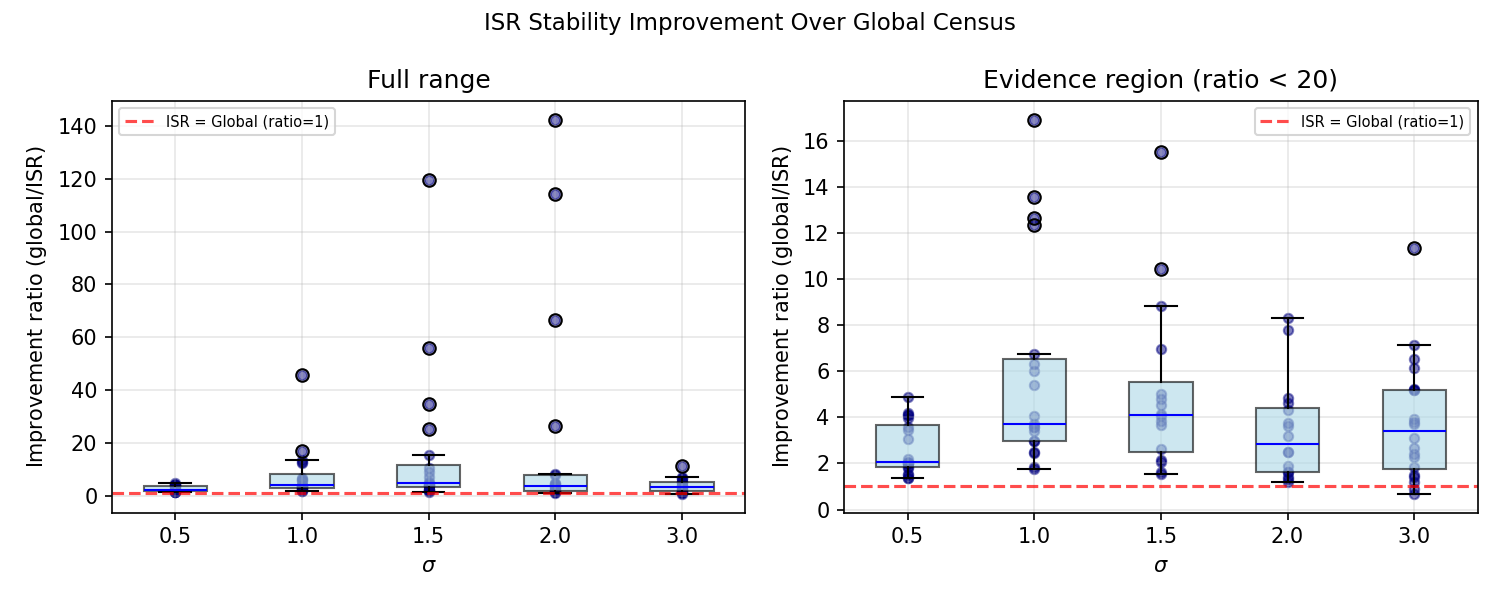
\includegraphics[width=\columnwidth]{figures/fig_07_stress_improvement_by_sigma.png}
  \caption{Improvement ratio $D_{\rm KL}^{\rm global} / D_{\rm KL}^{\rm ISR}$
  by $\sigma$. Points above 1 (dashed red line) indicate \ISR outperforms
  global. Boxes show quartiles across 20 seeds per $\sigma$.}
  \label{fig:stress_improvement}
\end{figure}

\subsection{Claim 4: Locality has basin-boundary exceptions}

The configuration-space locality diagnostics (Fig.~\ref{fig:basin_exception})
reveal that locality is not uniformly respected.
Using initial-field distance, the basin-exception rate rises from 5\% at
threshold 0.1 to 52\% at threshold 2.0 (Fig.~\ref{fig:basin_exception}).
This means that as we widen the ``nearby'' definition, more sectors that are
close in initial field value lie in different vacuum basins.

\begin{figure}[t]
  \centering
  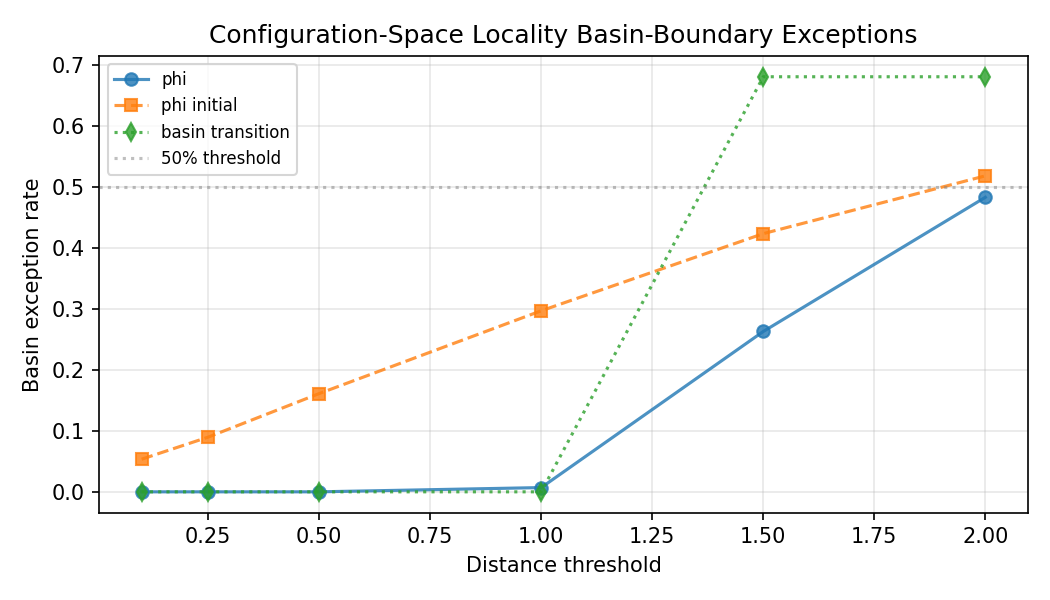
\includegraphics[width=\columnwidth]{figures/fig_05_basin_exception_rate.png}
  \caption{Basin-exception rate vs. distance threshold for three distance
  metrics. The initial-field metric (dashed) shows the most gradual rise,
  making it the most relevant diagnostic for locality continuity.}
  \label{fig:basin_exception}
\end{figure}

The continuity score (fraction of near same-basin pairs with small $\theta$
difference) is 1.0 for all thresholds: when sectors are in the same basin,
their effective physics is identical by construction.
Locality failures (near same-basin pairs with different $\theta$) are zero
for the same reason.
The relevant failure mode is the basin exception---nearby sectors in
different basins---which is captured by our diagnostics.

\subsection{Claim 5: Kernel-weighted sector averaging}

The kernel-weighted sector averaging (Table~\ref{tab:effective_coefficients}
in Appendix~\ref{app:supplementary}) shows aggregate coefficients as a
function of $\ell$.
At $\ell = 0.1$, the aggregate $\Lambda_{\rm eff} = 2.0$,
reflecting near-pure $x_0$ basin.
At $\ell = 2.0$, $\Lambda_{\rm eff} = 1.44$, shifted by mixing with
unobserved-sector vacua.
This averaging is a numerical consequence of the assigned physics vectors
$\boldsymbol{\theta}(v)$ and the kernel weighting; it is illustrative
of how sector weighting changes aggregate toy parameters in a
controlled toy setting, not a derivation of physical running couplings.

\subsection{Claim 6: Ell sensitivity reveals a sweet spot}

\begin{figure}[htbp]
  \centering
  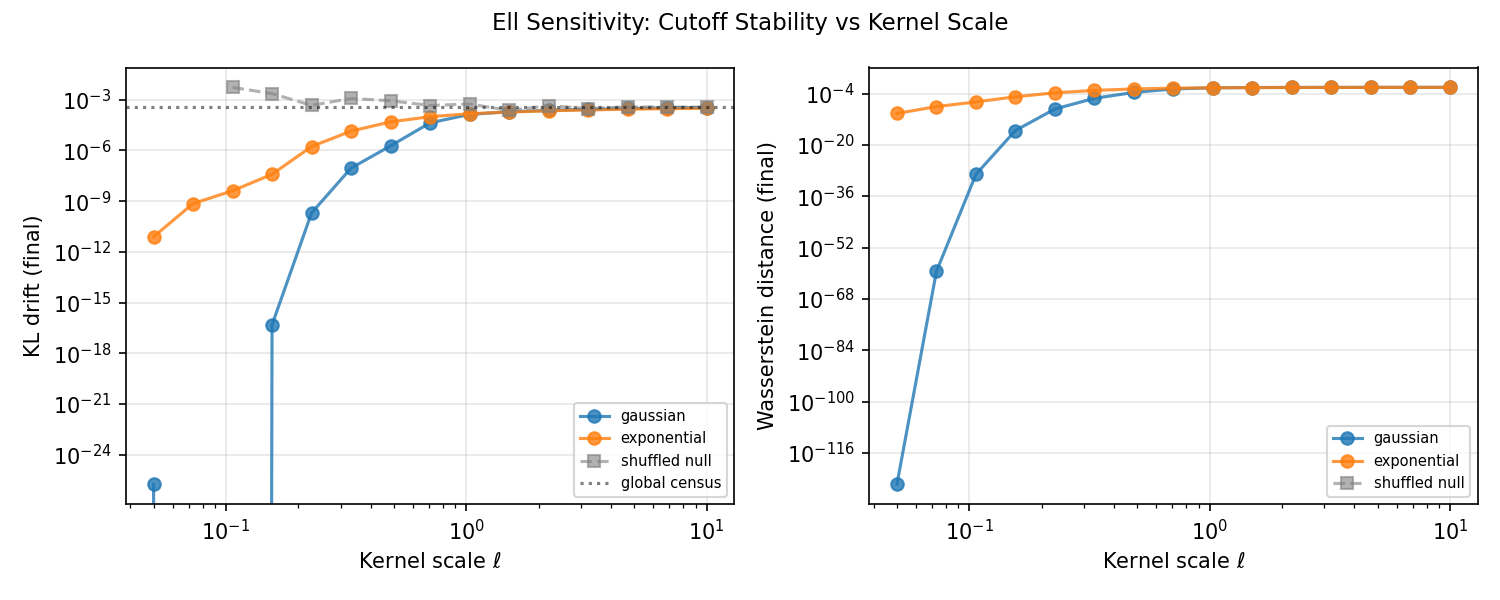
\includegraphics[width=\columnwidth]{figures/fig_11_ell_sensitivity_kl.png}
  \caption{KL drift and Wasserstein distance vs.\ kernel scale $\ell$.
  The black dotted line is the global-census baseline; the gray dashed
  line is the shuffled null control.}
  \label{fig:ell_sensitivity_kl}
\end{figure}

Fig.~\ref{fig:ell_sensitivity_kl} shows the evolution of ISR stability
metrics across $\ell$ (see Table~\ref{tab:ell_sensitivity} in
Appendix~\ref{app:supplementary} for the full data).
We define $N_{\rm eff} = (\sum_i w_i)^2 / \sum_i w_i^2$,
where $w_i = K_\ell[d(x_i, x_0)]$; $N_{\rm eff} \approx N$ when the kernel
weights all sectors equally and $N_{\rm eff} \ll N$ when only a few sectors
dominate.
Three regimes emerge:

\begin{itemize}
  \item \textbf{Narrow kernel} ($\ell \lesssim 0.2$): $N_{\rm eff} \ll N$,
        KL drift is vanishingly small (below $10^{-25}$ for $\ell=0.05$).
        This is an artifact: the kernel isolates only the
        $x_0$ basin and the ISR distribution is nearly a delta function.
        Reported KL divergences in this regime are not meaningful indicators
        of physical stability (see Appendix~\ref{app:degenerate}).
  \item \textbf{Sweet spot} ($0.5 \lesssim \ell \lesssim 1.5$):
        $N_{\rm eff} \approx 0.3$--$0.9\,N$, KL drift is $2$--$3\times$
        below global census, and basin exceptions remain below 30\%.
        The convergence rate $d(\log{\rm KL})/d(\log N) \approx -1.0$,
        comparable to global census.
  \item \textbf{Broad kernel} ($\ell \gtrsim 3$): $N_{\rm eff} \approx N$,
        KL drift approaches the global census value, and basin exceptions
        saturate above 60\%. ISR reduces to global weighting.
\end{itemize}

The randomized-distance null control (shuffled sector--distance pairings)
produces KL drift that always exceeds the correctly paired ISR at the same
$\ell$ and is typically comparable to or larger than the global-census
baseline.
This shows that the improvement is not a generic artifact of kernel smoothing;
it depends on preserving the field-space distance structure encoded by the
toy landscape.

\subsection{Claim 7: ISR remains favorable in the non-degenerate sigma--ell region}

\begin{table}[htbp]
  \centering
  \caption{Sigma-by-ell boundary: mean improvement ratio (global KL / ISR KL)
  across 5 seeds per cell, non-degenerate regime ($\ell \ge 0.50$).
  The degenerate small-$\ell$ columns ($\ell=0.10, 0.25$) are reported in
  Appendix~\ref{app:degenerate}.}
  \label{tab:sigma_ell_boundary}
  \small
  \begin{tabular}{lccc}
    \toprule
    $\sigma \backslash \ell$ & 0.50 & 1.00 & 2.00 \\
    \midrule
    0.5 & 68.5 & 3.12 & 1.28 \\
    1.0 & 142.5 & 5.97 & 1.86 \\
    1.5 & 240.0 & 5.38 & 2.35 \\
    2.0 & 103.1 & 7.68 & 4.40 \\
    3.0 & 58.5 & 6.27 & 2.46 \\
    \bottomrule
  \end{tabular}
\end{table}


\begin{figure}[htbp]
  \centering
  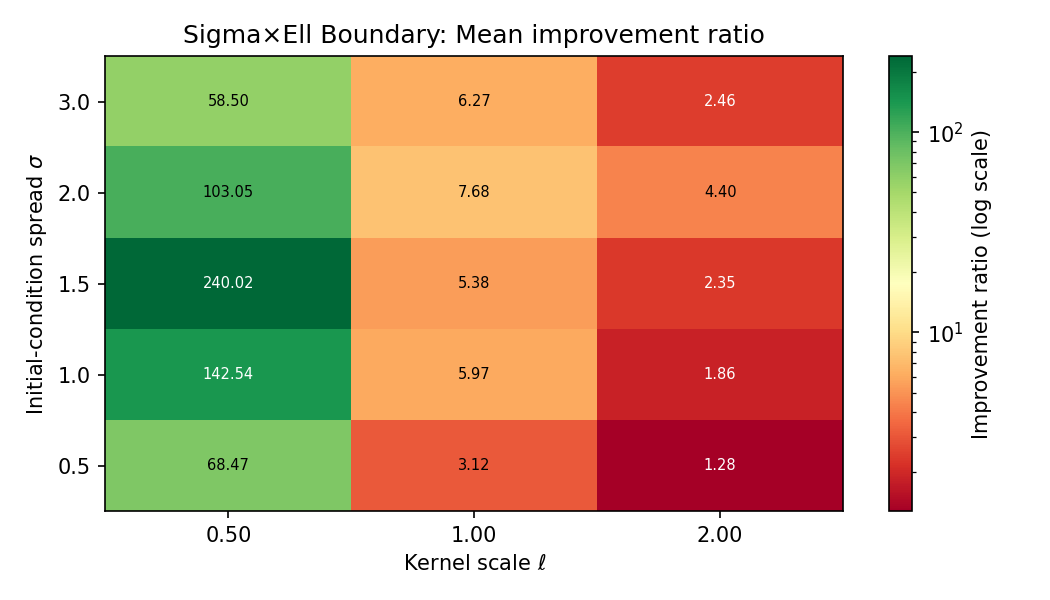
\includegraphics[width=\columnwidth]{figures/fig_13_sigma_ell_mean_improvement.png}
  \caption{Mean improvement ratio (global KL / ISR KL) across the sigma--ell
  grid. All non-degenerate cells ($\ell \ge 0.50$) exceed 1.}
  \label{fig:sigma_ell_boundary}
\end{figure}

The sigma--ell boundary experiment (Experiment~\ref{exp:10}) is a separate
scan from the 100-run stress test (Experiment~\ref{exp:8}).
Table~\ref{tab:sigma_ell_boundary} summarizes the non-degenerate region
($\ell \ge 0.50$) of the sigma--ell grid
(5 sigma values $\times$ 3 ell values $\times$ 5 seeds).
The improvement ratio remains $1.3$--$270$, with no failure case (ISR
underperforming global census) across any tested sigma--ell cell.
ISR improves over global census in \emph{every} tested non-degenerate cell of
the grid (improvement ratio $>1$).
The improvement is strongest at large $\sigma$ (broad initial-condition spreads),
where the global census is most cutoff-dependent.
Degenerate small-$\ell$ results ($\ell=0.10, 0.25$) are reported in
Appendix~\ref{app:degenerate}.

\subsection{Claim 8: ISR improvement is robust to landscape perturbation}

The landscape perturbation test (Experiment~\ref{exp:12}) shifts all well
centers by $+0.5$ while preserving the number of basins and physics vectors.
Table~\ref{tab:landscape_perturbation} shows the mean improvement ratio across
5 seeds.
In this limited perturbation test, ISR improves over global census in all
tested runs (all ratios $>1$), with qualitatively similar performance to
the unperturbed landscape.
The perturbation suggests that ISR improvement is not solely an artifact of
the original well placement.

\begin{table*}[t]
  \centering
  \caption{Landscape perturbation robustness: mean improvement ratio (global KL / ISR KL) for shifted well positions ($\mu \to \mu + 0.5$), 5 seeds per cell. ISR improves over global census in all tested runs (all ratios $>1$).}
  \label{tab:landscape_perturbation}
  \small
  \begin{tabular}{lccc}
    \toprule
    Landscape & $\sigma$ & Mean improvement ratio & Range \\
    \midrule
    Original & 1.5 & 11.3 & 2.0--32.9 \\
    Perturbed & 1.5 & 6.2 & 2.2--13.1 \\
    Perturbed & 3.0 & 7.0 & 1.9--20.6 \\
    \bottomrule
  \end{tabular}
\end{table*}

